\documentclass[11pt, a4paper]{article}
\usepackage[utf8x]{inputenc}
\usepackage[sort]{natbib}

\usepackage[spanish]{babel}
\usepackage{enumitem}
\usepackage{graphicx}
\usepackage{float}
\usepackage[linktoc=all]{hyperref}

\usepackage{etoolbox}

\usepackage{amsmath}
\usepackage{amssymb}
\usepackage{array}
\usepackage{gensymb}

\usepackage{fancyhdr}
\usepackage[table]{xcolor}
\usepackage{color}
\usepackage{colortbl}
\definecolor{lightgray}{gray}{0.9}
\setlength{\columnsep}{0.5cm}


%------------------- Dimensiones -------------------
\usepackage{geometry}
 \geometry{a4paper,total={170mm,257mm},left=15mm,right=15mm,top=20mm,}
%----------------------------------------------------

%------------------- Encabezado y Pie de pág -------------------
\pagestyle{fancy}
\fancyhf{}
\lhead{Técnicas Digitales IV}
\rhead{TP1}
\rfoot{Página \thepage}
%----------------------------------------------------


%----------------------------- Documento -----------------------------------------------
\begin{document}
\begin{titlepage}
 \centering
	
\includegraphics[scale=0.80]{Imagenes/LOGO.jpg} \par
 	\vspace{1cm}
 	{\scshape\LARGE Universidad Tecnológica Nacional \par}
 	{\scshape\large Facultad Regional de Córdoba \par}
 	\vspace{1cm}
	{\bfseries \Large Trabajo Práctico De Laboratorio $N^{\circ} 3$\par}
 	\vspace{1.5cm}

	\begin{tabular}{ll}
		Navarro, Facundo		&	63809 	
	\end{tabular}
	
	\vspace{1cm}
	Curso: 6r4 \\
	Grupo $N^{\circ} 5$
 	\vfill
	{\bfseries \Large Técnicas Digitales IV\par}

	\vspace{1.5cm}
	Docentes: \par
	Ing. Cayuela, Pablo \par
	Ing. Olmedo, Sergio \par

 	\vfill
	{\large \today\par}
\end{titlepage}
	
	
\tableofcontents
\clearpage

\section{Introducción}
	En este practico tiene como objetivo embeber un procesador dentro de la FPGA, en este caso se utilizo el softcore ``PicoBlaze".  PicoBlaze es la designación de una serie de tres gratuitas procesador suaves (softcore) núcleos de Xilinx para su uso en sus FPGA y CPLD productos. Se basan en una arquitectura RISC de 8-bit RISC y pueden alcanzar velocidades de hasta 100 MIPS en el Virtex 4 FPGA de la familia 7s. 

	Los procesadores tienen una dirección de 8 bits y puerto de datos para acceso a una amplia gama de periféricos. La licencia de los núcleos permite su uso gratuito, aunque sólo en los dispositivos de Xilinx, y vienen con herramientas de desarrollo . Herramientas de terceros están disponibles en Mediatronix y otros. El PauloBlaze es una implementación VHDL código abierto bajo la licencia Apache .

	El diseño original fue nombrado PicoBlaze KCPSM que significa "constante (K) con código programable Máquina de Estado" (antes "de Ken Chapman PSM"). Ken Chapman fue el diseñador de sistemas de Xilinx que ideó e implementó el microcontrolador.

\section{Desarrollo}
	Realizar  un proyecto donde integre el ejemplo de interrupciones de la documentación del KCPSM6 en VHDL. El archivo principal KCPSM.vhd contiene la descripción de uso libre de un CPU llamado Picoblaze, diseñado por el Ing. Ken Chapman de la empresa Xilinx. 

	\subsection{Estructura del proyecto}
		El proyecto fue desarrollado en el SW Vivado 2019.2.1 ya que se utilizó la plataforma de entrenamiento de Digilent, Basys3.

		\begin{figure}[H]
			\centering
			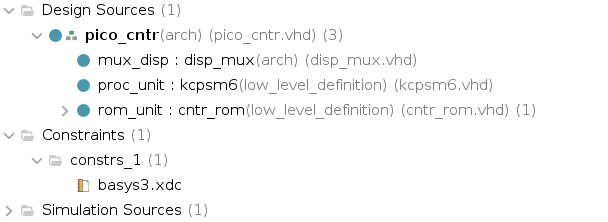
\includegraphics[width=0.6\textwidth]{Imagenes/proy-tree.png}
			\caption{Árbol del proyecto.}
			\label{fig:pry-tree}
		\end{figure} 

	\subsection{Desarrollo}
	Para poder utilizar el softcore PicoBlaze es tan simple como instanciar el archivo HDL provisto del sitio web de Xiling, consigo trae una serie de herramientas para generar el archivo ROM.vhd necesario que contendrá el código ensamblador en .psm correspondiente para el microcontrolador. En la figura \textcolor{blue}{\textbf{\ref{fig:kcpsm6_inst}}} se puede observar los dos modulos HDL de top-level, el módulo KCPSM6 y la ROM de instrucciones. 

		\begin{figure}[H]
			\centering
			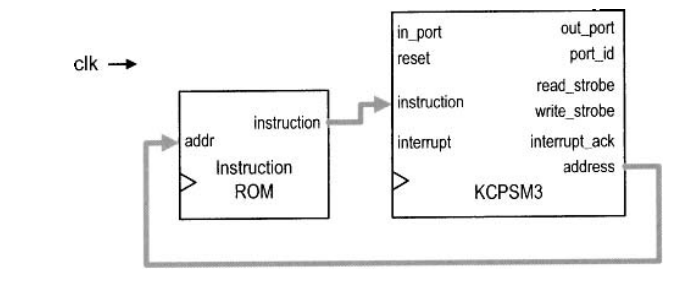
\includegraphics[width=0.6\textwidth]{Imagenes/top-level.png}
		\end{figure} 
		
		\begin{figure}[H]
			\centering
			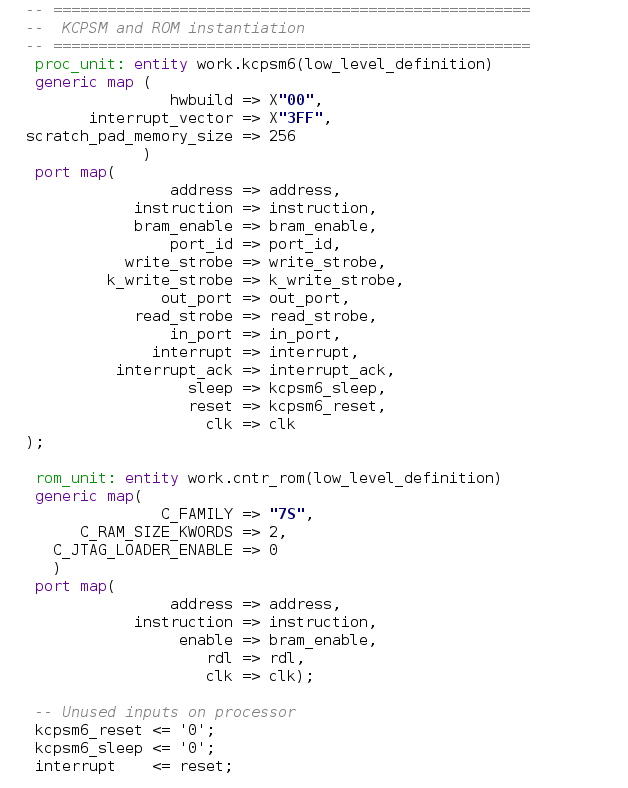
\includegraphics[width=0.6\textwidth]{Imagenes/kcpsm6_inst.png}
			\caption{Instansiacion de ROM y Core.}
			\label{fig:kcpsm6_inst}
		\end{figure} 

	\subsection{Codigo en PSM}
	Debido a su simplicidad, PicoBlaze no puede soportar lenguajes de programacion de alto nivel, y el desarrollo de codigo es en general desarrollado en lenguaje ensamblador. El metodo desarrollado fue el de "divide y conquistaras", de modo que se plantea un programa principal el cual llama a distintas funciones que ejecutan una tarea en particular, tal como se observa en \textcolor{blue}{\textbf{\ref{fig:asm_top}}}
		
		\begin{figure}[H]
			\centering
			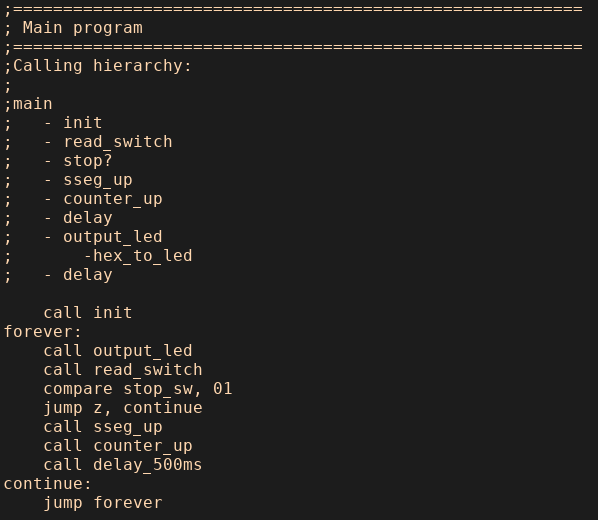
\includegraphics[width=0.4\textwidth]{Imagenes/asm-top.png}
			\caption{Estructura divide and conquer.}
			\label{fig:asm_top}
		\end{figure} 
	
	Para la generacion del .vhd necesario para instanciar en el Vivado, Xilinx provee una serie de herramientas que se pueden ver en \textcolor{blue}{\textbf{\ref{fig:tools}}}, el compilador kcpsm6 fue ejecutado en Linux a traves de ``wine"

		\begin{figure}[H]
			\centering
			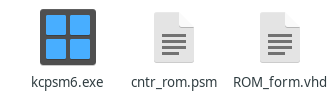
\includegraphics[width=0.4\textwidth]{Imagenes/tools.png}
			\caption{Archivos necesarios para compilar una ROM para PicoBlaze.}
			\label{fig:tools}
		\end{figure} 
		
	
	\subsection{Interrupciones}
	PicoBlaze es capaz de manejar interrupciones para circuitos externos de I/O, en nuestro caso como se vio en la instansiacion del CPU, la memoria de interrupcion esta ubicada en 3FF, tanto la llamada como la inicializacion se ve en la figura \textcolor{blue}{\textbf{\ref{fig:isr}}}

		\begin{figure}[H]
			\centering
			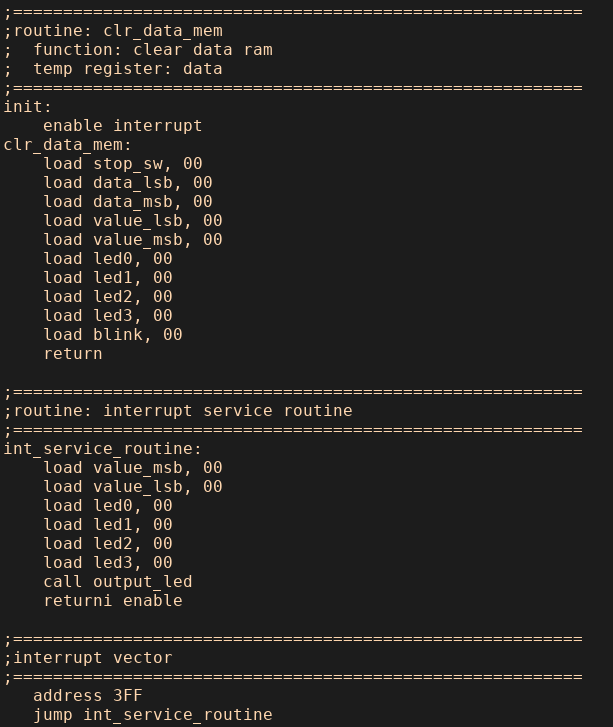
\includegraphics[width=0.4\textwidth]{Imagenes/isr.png}
			\caption{Habilitacion y llamada de interrupciones.}
			\label{fig:isr}
		\end{figure} 


\clearpage
	\subsection{Salida leds siete segmentos}
	La salida del contador se realiza tanto en los leds provistos por la placa como por los 7 segmentos, la decodificacion del numero en binario a bcd es realizado por el codigo ensamblador. En la figura \textcolor{blue}{\textbf{\ref{fig:sseg}}}
 
		\begin{figure}[H]
			\centering
			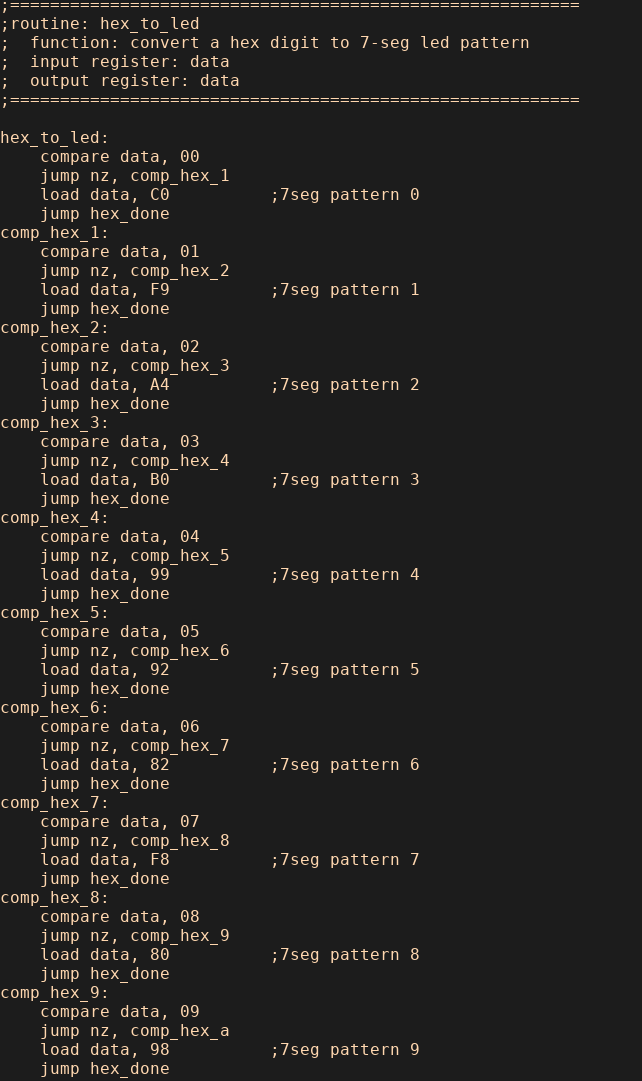
\includegraphics[width=0.4\textwidth]{Imagenes/sseg.png}
			\caption{Decodificación a nivel de software.}
			\label{fig:isr}
		\end{figure} 

\section{Multimedia}
		Se adjunta un dos links de unos vídeos demostrativos: 
		\begin{itemize}
			\item Presentación: \url{https://youtu.be/RMeyCFNI-uY}
			\item Demo: \url{https://youtu.be/nITNLCbS1TU}
		\end{itemize}

\end{document}
